% !TeX root = ../thesis.tex


\chapter{基本设计思路}
\section{项目简介}
芮总布置<基于消息调度的RTOS>是希望我们增强coding能力,因此我们小组决定从最简单的XV6开始学习,在弄懂最基本的操作系统概念之后,就在XV6上移植实时性相关算法,使其变成一个RTOS。同时XV6只是一个最简单的OS,我们或许会添加其他的功能,来完善它。{\color{red} 我们把这个项目当作为工作之余的兴趣爱好,作为一个兴趣小组来学习。因此,项目计划时间表不仅仅是五个周。}

目前规划了以下三个大的阶段:

1 学习XV6,达到手写操作系统中核心代码的能力

2 调研学习RT算法,动手改造XV6,使其成为RTOS

3 烧写RT-XV6到开发板中,完成整个开发流程


%\section{XV6基本介绍}
%\section{RTOS基本介绍}
\section{项目需求}
随着研究的深入,会慢慢完善各个需求点。

kernel内核启动过程需求

线程管理需求

线程间通信与同步需求 

内存管理需求

中断管理需求
\section{项目任务分解}
项目人员: 房继亮,许丽,廖章锦,顾权,赵林强
\subsection{了解调度器任务切换时保存现场信息的实现}
项目人员: 顾权
RTOS核心是任务管理,多任务的管理需要调度器来完成任务的切换,负责在何时去执行相应的任务。每个任务进程都有属于自己的进程属性块,保存着进程pid、当前使用的资源等信息。因此,在任务切换时需要保存自己内存和寄存器等现场信息,同时读取待运行进程的现场信息,完成上下文切换,让任务从上次退出的地方继续运行,完成任务切换的无缝衔接,实现任务的并发处理。

任务切换是RTOS的核心之一,现场信息的正确保存时实时操作系统正常运行的保障。
1. 学习xv6系统源码,了解需要保存哪些现场信息
2. 本系统是基于RISCV的RTOS,因此当调度器进行任务切换时,利用RISCV汇编代码高效的保存当前任务的现场信息
\subsection{了解进程切换函数中现场信息的切换}
项目人员:许丽
一个CPU看上去都像是在并发的执行多个进程,这是通过处理器在进程间切换来实现的,操作系统实现这种交错执行的机制称为上下文切换。当操作系统决定要把控制权从当前进程转移到某个新进程时,就会进行上下文切换,即保存当前进程的上下文,恢复新进程的上下文,然后将控制权传递到新进程,新进程就会从上次停止的地方开始。
上下文切换可以认为是内核(操作系统的核心)在 CPU 上对于进程(包括线程)进行以下的活动:
(1)挂起一个进程,将这个进程在 CPU 中的状态(上下文)存储于内存中的某处
(2)在内存中检索下一个进程的上下文并将其在 CPU 的寄存器中恢复
(3)跳转到程序计数器所指向的位置(即跳转到进程被中断时的代码行),以恢复该进程。
操作系统保持跟踪进程运行所需的所有状态信息,这种状态,也就是上下文,它包括许多信息,例如PC和寄存器文件的当前值,以及主存的内容。RTOS需要尽可能的缩小进程切换时间,保证实时性、可靠性。

\subsection{学习文件系统}
项目人员:房继亮
文件系统的目的是组织和存储数据,典型的文件系统支持用户和程序间的数据共享,且重启之后数据仍然可用。XV6的文件系统的文件、文件描述符、目录和路径类似Unix系统,并且把数据存储到一块IDE磁盘上,能够解决一些常见问题。XV6文件系统采用了分层的实现,大致包括块缓冲层、日志层、i节点、目录层、文件描述层,下面的每一层都提供接口供上层调用,XV6层级实现如下图\ref{fig:figfjl01}所示:
\begin{figure}[!htb]
	\centering
	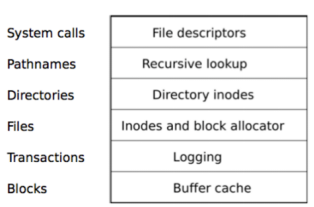
\includegraphics[width=0.9\linewidth]{figfjl01.png}
	\bicaption
	{文件系统} % 中文名
	{file system}  % 英文名
	\label{fig:figfjl01}
\end{figure}

\subsection{完成xv6 lock 和 scheduling 理论知识研究}
项目人员:赵林强
lock:分析xv6源码,输出包含锁机制实现原理和流程图的文档,并梳理出其关键代码。
file system:分析xv6源码,输出包含系统文件组成及其如何组织和存储数据的文档。
\subsection{完成对page table 和 traps 部分的实际代码研究}
项目人员:廖章锦

首先完成页表功能的理论分析,接着对xv6的原生代码进行了解,理解xv6页表每个功能的源码,最后完成对xv6源码的改进。

完成对代码的分析之后进行响应效率的改进

\section{调研学习RT算法,动手改造XV6,使其成为RTOS}
项目人员: 曾萧

研究RT算法,再xv6 OS的基础上,融入一个比较典型的RT算法。
\subsection{RT算法分类,典型特点,典型实现}
\subsection{RT算法研读,分享}
\subsection{RT算法移植}


\section{烧写RT-XV6到开发板中,完成整个开发流程}
项目人员:徐航
\subsection{掌握烧写流程及烧写工具的使用}
研究ROM中的BIOS程序,掌握系统启动时硬件初始化以及bootloader加载过程。当bootloader加载完成后由其引导操作系统启动。Bootloader负责时钟设置、硬件及必要设备初始化、检测系统内存映射、加载内核映像和根文件系统映像、设置内核的启动参数、启动内核等。
\subsection{烧写XV6到X86架构开发板}
在开发板上安装改造好的XV6系统,或在ubuntu系统中安装qemu+xv6
